% SIGIR 2027 submission (ACM Reference Format, sigconf, double-blind review)
% Build: pdflatex main && bibtex main && pdflatex main && pdflatex main
\documentclass[sigconf,review,anonymous]{acmart}

\setcopyright{none}
\settopmatter{printacmref=false}
\renewcommand\footnotetextcopyrightpermission[1]{}
\pagestyle{plain}

\usepackage{booktabs}
\usepackage{multirow}
\usepackage{graphicx}
\usepackage{amsmath}
\usepackage{xcolor}
\usepackage{subcaption}
\setlength{\emergencystretch}{1.5em}

\acmConference[SIGIR '27]{Proceedings of the 50th International ACM SIGIR Conference on Research and Development in Information Retrieval}{July 2027}{Padua, Italy}
\acmBooktitle{Proceedings of the 50th International ACM SIGIR Conference on Research and Development in Information Retrieval (SIGIR '27)}

\begin{document}

\title{Show the Path, Not the LLM: A 0.19B Path-Conditioned Reranker that Upgrades Any KGQA Retriever}

\author{Anonymous Author(s)}
\affiliation{\institution{Anonymous Institution}\country{}}

\begin{abstract}
Knowledge-graph question answering (KGQA) at the frontier is built on 7B-scale language models that generate relation paths over a question subgraph. These paths are expensive to produce, yet their value for \emph{ranking} the resulting candidates has never been isolated. We show that most of the ranking benefit can be obtained by simply \emph{showing the path} to a very small verifier. A 0.19B RWKV-7 cross-encoder, conditioned on \texttt{(question, relation path, candidate)}, is trained listwise in about seven minutes on a single GPU and used as a drop-in reranker.
Under a controlled protocol with identical training data, identical recipe and identical test pool, path conditioning lifts top-1 accuracy from 46.8 to 54.9 on WebQSP ($+8.1$ over three seeds; the same-seed paired test gives $+6.6$, $p=2.1\times10^{-10}$) and from 56.2 to 88.8 on MetaQA ($+32.7$ over two full-test seeds; the paired test on the 2{,}000-question subset, where both twins were originally evaluated, gives $+32.6$, $p=6.2\times10^{-142}$). The same verifier, applied \emph{without} retraining to the candidate sets of a 7B LLM retriever (RoG), raises its top-1 from 60.9 to 66.1 ($+5.2$, $p=8.5\times10^{-7}$) and, with RoG's own reader held fixed, lifts end-to-end accuracy from 73.8 to 75.6 ($p=4.2\times10^{-4}$); when the retriever doubles its candidate pool, its own count-based ranking collapses from 60.9 to 47.7 while ours holds at 66.7 ($+18.9$).
Insertion costs $+26$\,ms and $+2.2$\,GB per query because a cross-encoder scores all candidates of a question in one batched forward pass, something an autoregressive generator cannot do. We also delimit when the signal works: it degrades with path length ($+18.2$ on 1-hop vs.\ $+3.5$ on 2-hop WebQSP questions) and in magnitude across datasets ($+32.7$ MetaQA, $+6.6$ WebQSP, $+1.9$ CWQ), and on a large-vocabulary KG a coarse relation-\emph{type} summary of the path is enough (28.27 vs.\ 28.32 for the full chain); it transfers to a second, graph-based host only where that host's pool is recall-oriented, not where the host already ranks a short list well ($-1.9$). Code, checkpoints, per-question result files and all negative results are released in an anonymized repository.
\end{abstract}

\ccsdesc[500]{Information systems~Question answering}
\ccsdesc[500]{Information systems~Retrieval models and ranking}
\ccsdesc[300]{Computing methodologies~Knowledge representation and reasoning}

\keywords{knowledge graph question answering; reranking; relation path; resource-efficient IR; RWKV}

\maketitle

%% ---------------------------------------------------------------- 1
\section{Introduction}
\label{sec:intro}

Multi-hop knowledge-graph question answering (KGQA) is usually decomposed into retrieval and reasoning. The strongest recent systems place a 7B-parameter language model at the centre: RoG~\cite{luo2024rog} has the LLM plan relation paths over the question subgraph and then reason over the retrieved triples, reaching 81.5\% H@1 on WebQSP. Smaller transductive systems such as NSM~\cite{he2021nsm} (110M) and KGT5~\cite{saxena2022kgt5} (60M) avoid the LLM but require a dense entity table or an entity-linking pipeline.

This paper starts from a narrower question: \emph{given a candidate set produced by any retriever, what is the cheapest signal that reliably improves top-1 ranking?} Our answer is the relation path that the retriever already followed to reach each candidate---a short string that most rerankers discard.

We instantiate the idea as a 0.19B RWKV-7~\cite{peng2023rwkv,peng2025rwkv7} cross-encoder that scores \texttt{(question, relation path, candidate)} with a linear head. It shares its backbone with our own graph walker, adds no parameters at inference, trains listwise in roughly seven minutes on one RTX~4090, and can be dropped onto the candidate set of a completely different retriever without any modification of that retriever. We call the resulting system \textsc{GooseRAG}.

\paragraph{What we find.}
\begin{enumerate}
\item \textbf{Path conditioning is the dominant ranking signal.} Holding the training data, the recipe, the candidate pool and the scoring rule fixed (a ``twin'' control we introduce in \S\ref{sec:twin}), adding the path to the prompt lifts H@1 by $+8.1$ points on WebQSP and $+32.7$ on the full MetaQA test set.
\item \textbf{The verifier is portable across retrievers, within a measured boundary.} Trained on our walker's candidates, it reranks RoG-7B's candidates with no retraining: $60.9\to66.1$ ($+5.2$, $p=8.5\times10^{-7}$). With RoG's own reader held fixed, the same reranking raises end-to-end accuracy from 73.8 to 75.6 ($p=4.2\times10^{-4}$). When RoG emits twice as many candidates its own ranking collapses to 47.7, while ours stays at 66.7 ($+18.9$): extra recall is only realised by a competent reranker. On a \emph{graph} host with a short, high-precision pool the transfer does not pay ($-1.9$ against GNN-RAG's own in-domain score), which locates the boundary at recall-oriented candidate sets (\S\ref{sec:portable-results}).
\item \textbf{Insertion is cheap.} A cross-encoder performs one forward pass per candidate and no autoregressive decoding, so all candidates of a question are scored in a single batch: $+26$\,ms and $+2.2$\,GB on top of the host retriever. Scoring candidates one at a time would cost $+428$\,ms, which is what an LLM-based reranker is forced to do.
\item \textbf{The benefit has a quantitative boundary, and a prescription.} It shrinks with path length (1-hop: $+18.2$; 2-hop: $+3.5$ on WebQSP) and in magnitude across datasets ($+32.7$ MetaQA, $+6.6$ WebQSP, $+1.9$ CWQ), tracking positive density and relation-vocabulary size. Under a twin control on CWQ, a coarse relation-\emph{type} summary of the path recovers the entire gain of the full chain (28.27 vs.\ 28.32), while the first hop alone recovers half (\S\ref{sec:boundary}).
\item \textbf{The same verifier can buy back retrieval budget.} Guiding the beam with verifier scores leaves the standard beam untouched but lets a 20-wide beam match a 200-wide beam (56.12 vs.\ 56.18) at a tenth of the search.
\item \textbf{The gain is the path, not the backbone.} On the same pool, a BERT-base cross-encoder trained with the same objective and input gains $+11.9$ from the path, the same order of magnitude as our RWKV verifier ($+12.2$); all three trained sub-0.2B cross-encoders land within two points (55.3/56.6/57.2), a 0.5B decoder trained the same way reaches 59.8 (+3.3 over the best encoder), and the same 0.5B used zero-shot is near chance (7--9\%). The signal must be learned, and it keeps improving with capacity; we compete on cost, not on the accuracy frontier.
\end{enumerate}

\paragraph{What this is not.}
It is not a new architecture: the deployed system is a shared recurrent backbone, a path-conditioned prompt and a linear head. It is not state of the art: NSM (110M, 68.7\% on WebQSP as reported by its authors~\cite{he2021nsm}) dominates us on the parameter--accuracy plane. It is not the strongest reranker either: a BERT-base cross-encoder with the same path input ties or slightly beats ours, and a 0.5B decoder trained the same way beats both by three to five points (\S\ref{sec:external}). Our claim is about what the path is worth and how cheaply it can be plugged into another retriever, not about owning the best scorer. We report this explicitly, together with every negative result we obtained (\S\ref{sec:neg}).

%% ---------------------------------------------------------------- 2
\section{Related Work}
\label{sec:related}

\paragraph{Retrieval-then-reason KGQA.}
NSM~\cite{he2021nsm} learns a symbolic search over a dense entity table; KGT5~\cite{saxena2022kgt5} casts KGQA as sequence-to-sequence generation over entity titles; both are transductive. SR~\cite{zhang2022sr} and UniKGQA~\cite{jiang2023unikgqa} keep a retriever in the loop with a graph neural network. The current frontier uses an LLM to plan paths (RoG~\cite{luo2024rog}), retrieve a text subgraph, and reason over it; GNN-RAG~\cite{mavromatis2024gnnrag} replaces LLM planning with GNN retrieval and keeps the LLM for reasoning. Our layer sits \emph{downstream} of all of them: we neither plan paths nor reason, we rank the triples a retriever already produced. This is why a verifier trained on our walker transfers to RoG's candidate sets without retraining.

\paragraph{Path-based ranking and path planning.}
Scoring candidate answers with relation paths is an old idea: PRA~\cite{lao2011pra} and subgraph feature extraction~\cite{gardner2015subgraph} rank answers by the paths that reach them, and DeepPath~\cite{xiong2017deeppath} and Go for a Walk~\cite{das2018gowalk} learn path-finding policies with reinforcement learning. These methods \emph{search for} paths as part of inference. A second line uses paths as explicit reasoning traces: ToG~\cite{sun2024tog} lets an LLM agent beam-search over the KG, and FiDeLiS~\cite{sui2024fidelis} scores step-wise paths for faithful reasoning. Both remain planners that consume an LLM at inference. Our contribution is orthogonal: we take the path as \emph{given} by whatever retriever produced the candidate and measure, under a controlled protocol, how much a path-conditioned scorer adds at the ranking stage---and show that this scorer can be lifted onto another retriever's paths unchanged.

\paragraph{Reranking.}
Cross-encoders such as monoBERT~\cite{nogueira2019passage} and ColBERT~\cite{khattab2020colbert} score a (query, document) pair independently and are therefore portable but structure-blind; LLM listwise rerankers~\cite{sun2023rankgpt} buy context awareness with extra autoregressive calls. Dense retrieval and reranking pipelines~\cite{karpukhin2020dpr} assume flat text. Our verifier is a cross-encoder over \texttt{(question, relation path, entity)}: cheap per item, but conditioned on a structure that text rerankers never see, and independent of the retriever's own model.

\paragraph{What the path buys, and when.}
Prior KGQA rankers consume the whole subgraph or entity embeddings. We isolate a single string---the relation path---and quantify its role with control experiments: random-relation substitution, entity masking, hop-wise splits, a per-question dose--response analysis, and three datasets with different positive densities. The resulting operational boundary (positive density \emph{and} path length) is, to our knowledge, not previously stated in this form, and it is one of our contributions rather than a caveat.

\paragraph{Efficient backbones.}
RWKV~\cite{peng2023rwkv,peng2025rwkv7} provides a constant-size recurrent state, and hardware-efficient linear attention~\cite{yang2024fla} makes it practical. We use one 0.19B RWKV-7 as the shared backbone of walker and verifier; a long-context state-reuse advantage did \emph{not} materialise in current kernels (Appendix~\ref{app:longctx}), so we make no such claim.

%% ---------------------------------------------------------------- 3
\section{Method}
\label{sec:method}

\subsection{Shared backbone and graph walker}
\label{sec:walker}
The backbone is RWKV7-Goose-World2.8-0.1B (191M parameters). A relation head scores \texttt{(question, relation prefix)} $\rightarrow$ next relation and is trained with positives from gold paths and hard negatives---high-scoring wrong entities produced by a first verifier pass. Beam search (beam 200, top-15 relations per node, at most 128 children per relation, at most 2 hops, $\beta=2.0$, $\gamma=0.5$, generic relations banned) yields up to 200 candidates, each annotated with the relation sequence that produced it. On WebQSP the gold answer is inside this pool for 78.1\% of questions. This is a \emph{recall} quantity measured under one fixed walker configuration; being in the pool is necessary but not sufficient to be ranked first, and the remaining 21.9\% (344 questions, all with empty candidate pools) are unrecoverable at the ranking stage by construction.

\subsection{Path-conditioned verifier}
\label{sec:verifier}
Each candidate is scored by a single sequence:
\begin{quote}\ttfamily\small
Question: \{q\}\\
Relation path: \{r1 -> r2\}\\
Candidate: \{e\}\\
Is this the final answer?
\end{quote}
A linear head on the final hidden state produces $\mathrm{logit}[1]-\mathrm{logit}[0]$. Training is listwise within a question: a softmax over the candidates of that question followed by cross-entropy on the gold candidate(s). Two epochs suffice (7 minutes, one RTX 4090). The deployed system then fine-tunes the backbone end-to-end on the same objective for 3 epochs and keeps a single head, so walker and verifier share one set of 191M weights.

The path is rendered as a plain relation chain. \S\ref{sec:presentation} shows that the exact rendering barely matters: full Freebase names, namespace-stripped names, a natural-language sentence, and a chain with intermediate entities all fall within 1.6 points.\label{sec:presentation}

\subsection{Portable usage}
\label{sec:portable}
Given a candidate set from any retriever, we form the same triple from \emph{that retriever's} question, candidate and path, and sort by the verifier score. Nothing in the retriever is modified and no LLM is invoked. Because scoring a candidate is one forward pass with no autoregressive decoding, all candidates of a query are scored in a single batch (\S\ref{sec:cost}).

\subsection{Pre-registered protocol}
\label{sec:protocol}
All pipeline hyperparameters were fixed before the final test runs (beam 200, top-15 relations, 128 children, 2 hops, $\beta=2.0$, $\gamma=0.5$, verifier top 200). Test sets were evaluated once per configuration. Validation was used only to check feasibility: validation candidate pools contain at most 100 candidates by construction, and validation and test select pipeline parameters in opposite directions, so tuning on validation is not possible here (\S\ref{sec:neg}).

%% ---------------------------------------------------------------- 4
\section{Experimental Setup}
\label{sec:setup}

\paragraph{Datasets.}
WebQSP~\cite{berant2013webqsp} (2,812/245/1,628 train/val/test; we report 1,627 after dropping rows with empty answers), CWQ~\cite{talmor2018cwq} (3,520 test), and MetaQA~\cite{zhang2017metaqa} (vanilla 1/2/3-hop; we sample 3,807 training questions with a stride across hops, evaluate on all 14,274 test questions and on a 2,000-question subset for ablations).

\paragraph{Metrics.}
H@1 is primary. Operationally, each question has a gold set $G$ of answer entities and the system returns a ranked list; a question is correct iff the top-1 entity string is an element of $G$. Matching is exact on the entity names supplied by the dataset (the canonical names RoG uses), with no lower-casing, alias table, or fuzzy match; when a question has several gold answers, matching any one counts. H@$k$ and set-hit apply the same rule to the first $k$ items, and the in-pool oracle (gold $\in$ pool) separates recall from ranking. An empty candidate pool counts as a miss in the $n=1{,}627$ denominator.

\paragraph{Statistics.}
Paired comparisons use the exact McNemar test~\cite{mcnemar1947} on per-question binary outcomes of two systems evaluated on the same questions, plus 10{,}000-sample bootstrap 95\% confidence intervals~\cite{efron1979} on the accuracy difference. All reported $p$ values are uncorrected. The three headline comparisons (twin WebQSP, twin MetaQA, RoG portability) sit at $p\le 8.5\times10^{-7}$, far below a conservative Bonferroni threshold of $3\times10^{-3}$ ($\alpha=0.05$ over the $\sim$15 paired tests in this paper); the set-wise reranking comparison is weaker ($p=0.02$) and is treated as supportive rather than as a headline claim.

\paragraph{Systems compared.}
(i) walker score; (ii) plain verifier (no path); (iii) fused walker+verifier score; (iv) path-conditioned verifier; (v) the same verifier after backbone fine-tuning; (vi) set-wise reranking over frozen hidden states as a reference point; (vii) RoG-7B as a host retriever for portability; (viii) published numbers for NSM, KGT5, RoG; (ix) external rerankers trained on the \emph{same} groups and evaluated on the \emph{same} pool---a BERT-base cross-encoder (with and without the path), a T5-base encoder cross-encoder, and a 0.5B instruction-tuned LLM used as a zero-shot listwise reranker; (x) a reader-level end-to-end comparison in which the top-5 paths under two orderings are fed to the RoG-7B reader.

\paragraph{Hardware.}
All latency and memory numbers were measured on one RTX 4090 (24\,GB). Training runs were spread over that machine, an RTX 5090 and (for the revision experiments) an RTX 3090; re-running stored checkpoints on another GPU reproduces the reported accuracies within 0.5 points (Appendix~\ref{app:hw}), and every comparison in a table is computed on a single GPU and software stack. The FLA RWKV-7 kernels require CUDA and bf16.

%% ---------------------------------------------------------------- 5
\section{Results}
\label{sec:results}

\subsection{Main results}
\label{sec:main}

\begin{table}[t]
\centering\small
\caption{WebQSP test, cumulative (n=1,627; verifier top 200). Empty candidate pools count as misses; Table~\ref{tab:samepool} instead uses the 1,615 questions with a non-empty pool, which is why its figures are 0.3--0.4 points higher for the same systems.}
\label{tab:main}
\begin{tabular}{lr}
\toprule
System & H@1 \\
\midrule
Plain verifier + fused score (published baseline) & 44.19 \\
\quad + relation head (VGHN) & 47.94 \\
\quad + path-conditioned verifier & 56.12 \\
\quad + set-wise reranking (frozen states) & 57.22 \\
\quad \textbf{+ backbone fine-tuning (deployed)} & \textbf{58.03} \\
\bottomrule
\end{tabular}
\end{table}

Table~\ref{tab:main} shows the cumulative ablation on the full test set. The deployed system reaches H@5 = 72.0\% (mean over five seeds). Five seeds give $58.46\pm0.35$ on the 1,615 questions with a non-empty pool, i.e.\ 58.03 on all 1,627.

On MetaQA the path-conditioned verifier reaches 87.97\% with the original training set and $88.82\pm0.62$ with the twin recipe over all 14,274 test questions; the plain twin reaches $56.16\pm1.83$, i.e.\ $+32.7$ under identical data (\S\ref{sec:twin}). Set-hit is 99.61\%, so MetaQA measures ranking almost purely.

On CWQ the path verifier gains 1.90 points under a twin control (26.42 $\rightarrow$ 28.32, $p=1.4\times10^{-3}$), and a coarse relation-type summary recovers the same gain; \S\ref{sec:boundary} explains both.

\begin{figure}[t]
\centering
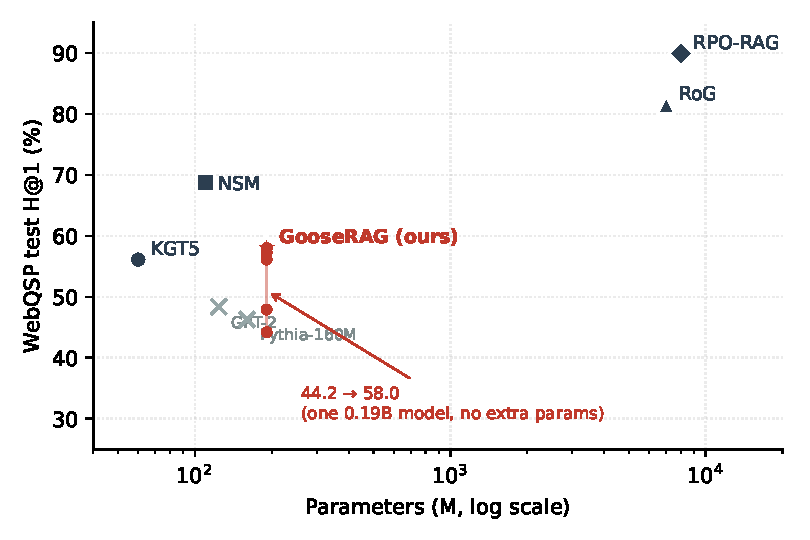
\includegraphics[width=\linewidth]{figures/fig1_pareto_params.pdf}
\caption{Parameter--accuracy plane on WebQSP. Our 0.19B system sits below NSM (transductive) but requires no entity table and no LLM; the two crosses are same-pool, same-recipe Transformer controls (GPT-2 124M, Pythia-160M).}
\label{fig:pareto}
\end{figure}

\subsection{A twin control for path conditioning}
\label{sec:twin}

Published comparisons of ``path vs.\ no-path'' verifiers usually change two things at once: the prompt \emph{and} the data the checkpoint was trained on. We therefore build a \emph{twin}: the same training groups, the same recipe, the same seed, the only difference being that the path is removed from the prompt.

\begin{table}[t]
\centering\small
\caption{Twin-controlled path conditioning (identical data, recipe, and test pool). Means $\pm$ std over seeds. MetaQA is the full 14{,}274-question test set; the 2{,}000-question subset used for the paired test gives $53.75$ vs.\ $88.98$ ($+35.2$).}
\label{tab:twin}
\begin{tabular}{llcc}
\toprule
Dataset & Verifier & Seeds & H@1 \\
\midrule
\multirow{2}{*}{WebQSP} & plain twin & 3 & $46.75\pm1.38$ \\
 & \textbf{path} & 3 & $\mathbf{54.89\pm0.12}$ \\
\midrule
\multirow{2}{*}{MetaQA (full)} & plain twin & 2 & $56.16\pm1.83$ \\
 & \textbf{path} & 2 & $\mathbf{88.82\pm0.62}$ \\
\bottomrule
\end{tabular}
\end{table}

Table~\ref{tab:twin} reports the result. On WebQSP the paired per-question test (same seed, $n=1{,}627$) gives $+6.58$ points, $b/c=89/196$, $p=2.1\times10^{-10}$, bootstrap CI $[+4.61,+8.60]$; averaging over three seeds gives $+8.14$. On MetaQA the headline is the full test set: $56.16\pm1.83$ (plain, 2 seeds) vs.\ $88.82\pm0.62$ (path, 2 seeds), $+32.66$. The paired per-question test was run on the 2{,}000-question subset on which both twins were first evaluated: $+32.60$, $b/c=61/713$, $p=6.2\times10^{-142}$, CI $[+30.3,+34.9]$. The subset is harder for the plain verifier ($53.75$ vs.\ $56.16$ on the full set) but the path verifier is stable ($88.98$ vs.\ $88.82$), which is why the subset effect ($+35.2$) is slightly larger than the full-set effect ($+32.7$).

Two remarks. First, the twin-controlled effect is smaller than the number obtained against the historical baseline ($+13.9$ on WebQSP), because that baseline was trained on a different, weaker candidate pool. We report the controlled number as our headline and keep the historical comparison only for continuity. Second, path conditioning also \emph{reduces the across-seed spread} by roughly an order of magnitude on WebQSP ($\pm0.12$ vs.\ $\pm1.38$, three seeds each); with three seeds we report this as a consistent pattern rather than a precisely estimated variance ratio.

\subsection{Same-pool single-variable ablation}
\label{sec:samepool}

Holding the candidate pool (top-200 from the relation-head mining) and the fusion rule fixed, and changing only the ranking function:

\begin{table}[t]
\centering\small
\caption{One candidate pool, five ranking functions (WebQSP, n=1,615).}
\label{tab:samepool}
\begin{tabular}{lccc}
\toprule
Ranking function & H@1 & H@5 & H@10 \\
\midrule
Walker score & 17.77 & 42.91 & 52.20 \\
Plain verifier & 41.98 & -- & -- \\
Fused (0.5$\cdot$walker + 2$\cdot$verifier) & 48.30 & -- & -- \\
\textbf{Path verifier} & \textbf{55.91} & 70.34 & 73.31 \\
Fused (path) & 56.59 & 70.71 & 73.87 \\
+ set-wise reranking (5 seeds) & $57.60\pm0.12$ & 70.93 & 74.14 \\
\bottomrule
\end{tabular}
\end{table}

Path conditioning is the largest single effect we observe (Table~\ref{tab:samepool}). Set-wise reranking over the verifier's frozen states adds a further $+1.0$ over the fused path score; removing cross-candidate attention costs only 0.11 points, so the gain comes from reusing the verifier's hidden state and within-question normalisation rather than from candidate interaction.

\subsection{Is this the best cheap reranker? External baselines on the same pool}
\label{sec:external}

A controlled path effect does not by itself show that our model is the best cheap reranker, so we train external rerankers on the \emph{same} groups with the \emph{same} listwise objective, the same candidate budget (64) and length (128), and evaluate them on the \emph{same} pool ($n=1{,}627$); only the backbone changes. Qwen is used zero-shot (no training) as a listwise reranker over the first 100 candidates, because its context cannot hold 200 paths; our verifier is re-scored on that same top-100 subset for the comparison.

\begin{table}[t]
\centering\footnotesize
\caption{External rerankers on one candidate pool (WebQSP test, $n=1{,}627$). Three trained sub-0.2B encoders land within two points; a 0.5B decoder trained with the same objective is 3.3 above the best of them, while the same model used zero-shot is near chance.}
\label{tab:external}
\begin{tabular}{lccc}
\toprule
Reranker & Params & no path & + path \\
\midrule
RWKV-7 (ours, shared with walker) & 191M & 43.02 & 55.26 \\
BERT-base cross-encoder & 110M & 44.62 & 56.55 \\
T5-base encoder cross-encoder & 110M & -- & 57.22 \\
Qwen2.5-0.5B, trained (same listwise objective) & 494M & -- & \textbf{59.80} \\
Qwen2.5-0.5B, zero-shot listwise (top-100) & 494M & 9.47 & 7.44 \\
\quad ours, same top-100 pool & 191M & -- & 53.29 \\
\bottomrule
\end{tabular}
\end{table}

Three findings. (i) \emph{The path effect belongs to the input, not to our backbone}: the same $\approx+12$ appears for BERT (+11.92, $p=2.2\times10^{-23}$, CI $[+9.6,+14.3]$) and for RWKV (+12.24). (ii) \emph{Accuracy scales with backbone capacity, not with our design}: the three trained sub-0.2B encoders land within two points of each other (55.3/56.6/57.2), BERT-base is 1.29 above ours without a separable difference ($p=0.19$, CI $[-0.6,+3.1]$), T5-base is 1.97 above (nominal $p=0.03$ uncorrected), and a 0.5B decoder-only model trained with the \emph{same} listwise objective and input reaches 59.80, i.e.\ $+3.26$ over BERT ($p=2.3\times10^{-4}$, CI $[+1.5,+4.9]$) and $+4.55$ over ours ($p=6.0\times10^{-7}$, CI $[+2.8,+6.3]$). We therefore do not claim the best reranker; the deployment argument for our model is accounting and latency: it shares the walker's 191M weights and scores all candidates in one batch, whereas a BERT, T5 or 0.5B decoder adds a second model and, for the decoder, an order of magnitude more compute per candidate. (iii) \emph{Zero-shot listwise prompting is not a substitute}: the \emph{same} 0.5B model reading the same candidates answers correctly in 7--9\% of questions when used zero-shot, against 59.8\% when trained, so the gain requires a trained scorer, not merely an LLM.

\subsection{Portability across retrievers}
\label{sec:portable-results}

\begin{table}[t]
\centering\footnotesize
\caption{RoG-7B as host retriever (WebQSP, n=1,628). The candidate set is fixed per row and only the ranking function changes.}
\label{tab:pluggable}
\begin{tabular}{lcccc}
\toprule
RoG beam & Cand./q & RoG-native & ours (frozen) & ours (fine-tuned) \\
\midrule
3 & 15.7 & 60.93 & 65.36 & \textbf{66.09} \\
10 & 30.3 & 47.73 & -- & \textbf{66.65} \\
\bottomrule
\end{tabular}
\par\vspace{3pt}
\footnotesize $\Delta$ vs.\ RoG-native: $+4.42$ (frozen, beam 3), $+5.16$ (fine-tuned, beam 3, $p=8.5\times10^{-7}$), $+18.92$ (fine-tuned, beam 10). Rows are ranking H@1 with the reader removed; the end-to-end check through RoG's own reader is in the text.
\end{table}

The candidate set is produced entirely by RoG; our verifier is trained only on our walker's candidates (``cross-retriever'' transfer). The beam-3 comparison is significant ($p=8.5\times10^{-7}$). The beam-10 row is the informative one: doubling the pool destroys RoG's count-based ranking ($-13.2$) while our verifier is essentially unchanged ($+0.6$). The $+18.92$ therefore combines two effects---our reranker is stable, and RoG's own ordering degrades---and the honest reading is that extra recall is only realised by a competent reranker, which is exactly the role we propose.

\begin{figure}[t]
\centering
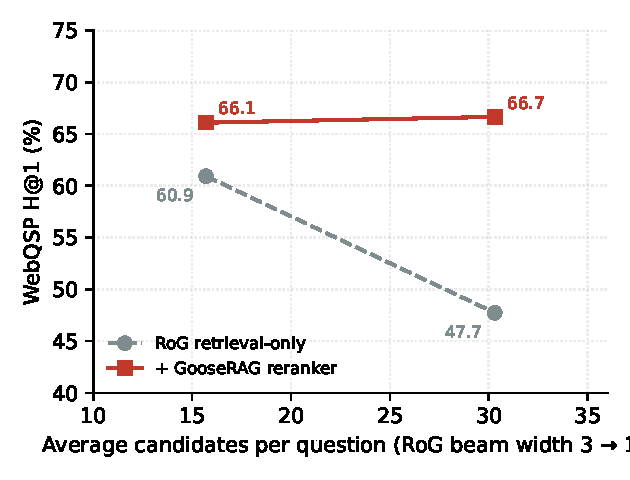
\includegraphics[width=0.95\linewidth]{figures/fig4_beam_scaling.pdf}
\caption{The host retriever's own ranking collapses when it emits more candidates; the path-conditioned verifier does not. Portability is therefore not a small-sample artefact.}
\label{fig:beam}
\end{figure}

Scope note: this table compares retrieval and reranking only. RoG's own pipeline, which also contains a 7B reader, reports 81.5\% H@1 end-to-end on WebQSP~\cite{luo2024rog}. We run that check separately rather than inside the table. Feeding the top-5 paths of both rankings to RoG's \emph{own} reader, unchanged, raises end-to-end accuracy from 73.77 to 75.55 ($+1.78$; exact McNemar $p=4.2\times10^{-4}$, discordant pairs 47/18, $n=1{,}628$), while the ranking-level H@1 on this pool moves from 61.55 to 66.40---the same direction and size as the frozen row of Table~\ref{tab:pluggable}, on a smaller pool (7.9 candidates per question). The absolute end-to-end level is below the 81.5\% reported for RoG because our replay of its beam-3 rules leaves 15.4\% of questions with an empty pool; the comparison is internal to this pool, with the same reader, the same candidates and only the ranking changed.

\paragraph{A second host, and where portability stops.}
RoG is a generative retriever with a large, noisy pool. To test whether the transfer is a property of the layer or of that host, we repeat it on a \emph{graph} retriever: GNN-RAG's released ReaRev-WebQSP checkpoint~\cite{mavromatis2024gnnrag}, whose pipeline is a GNN over a dense subgraph that emits candidate answer nodes with scores. We take its released per-question output on the WebQSP test split (our rerun of the checkpoint reproduces its reported H@1), recover each candidate's relation path by breadth-first search from the topic entities over the same subgraph (at most three hops; every candidate has a path), and apply the \emph{same} verifier with no retraining and no change to the host. The substitution is exact: same candidates, same question, only the ranking function changes, and matching is on Freebase ids, the native space of that release.

The result is negative, and informatively so. This pool is small and precise---8.1 candidates per question, gold present for 88.8\% of questions---and the host's own GNN score already ranks it at 76.23, whereas our zero-shot verifier reaches 74.32 ($-1.90$; exact McNemar $p=0.037$, $b/c=88/119$). Rank fusion of the two scores recovers the host exactly (76.29 vs.\ 76.23, $p=1$) but does not exceed it, and re-fitting the verifier on the host's own training split (2{,}703 groups, seven minutes) \emph{lowers} it to 73.77, because that split is 75\% positive and therefore carries almost no ranking signal. The loss is not uniform: splitting by pool size, we lose $3.66$ points where the host emits at most five candidates ($n=1{,}120$, $p=5.5\times10^{-5}$), lose 0.87 in the 6--10 bucket ($n=229$, $p=0.89$), and \emph{gain} $4.30$ where it emits more than ten ($n=279$, $p=0.14$). That ordering is the same quantity as our boundary rule (\S\ref{sec:boundary}): the path-conditioned scorer pays where the pool is recall-oriented and the host's own ordering is weak, and it does not pay where a strong, in-domain GNN has already ranked a short, high-precision list. We therefore state portability narrowly---\emph{any retriever whose candidate set is recall-oriented, i.e.\ large and noisy}---and report this host as the negative half of that boundary rather than dropping it.

\subsection{Cost and its structure}
\label{sec:cost}

\begin{table}[t]
\centering\small
\caption{Measured cost on one RTX 4090. Batching all candidates of a query is what a cross-encoder can do and a generator cannot.}
\label{tab:cost}
\begin{tabular}{lcc}
\toprule
 & Full system & Inserted as reranker \\
\midrule
Parameters & 191M & 191M (additional) \\
Latency, one batch per query & \textbf{278 ms} & \textbf{+26 ms} \\
\quad (beam 73 + scoring 205) & & (15.7 candidates) \\
Latency, serial per candidate & 3.9 s & +428 ms \\
Peak memory & 2.2 GB & +2.2 GB \\
External LLM & none & none \\
\bottomrule
\end{tabular}
\end{table}

Scoring 16 / 32 / 200 candidates takes 26.0 / 28.6 / 163.9 ms when batched, against 428 / 704 / 3,824 ms when scored one at a time. The batched figure is the deployment-relevant one: a verifier has no sequential dependency between candidates, while an LLM reranker must generate its judgement token by token. Inserting our layer therefore buys $+5.2$ points for about 4\% additional latency on top of the host's $\sim$620 ms.

A candidate-count sweep (25/50/100/200 scored candidates) gives 49.23/51.38/54.33/56.18 H@1 at roughly 0.8 ms per candidate: the method degrades gracefully when a host can only supply a small pool, which is precisely the regime of a beam-3 LLM retriever.

Finally, a verifier-guided beam---pruning each hop by verifier score instead of walker score---does nothing at beam 200 (60.50 vs.\ 60.50, measured on the first 400 questions, the subset on which a 200-wide sweep was affordable) but recovers most of the loss at narrow beams: on the full 1,627-question test set, beam 20 goes from 53.78 to 56.12 ($+2.33$), i.e.\ it matches the beam-200 result (56.18) with a tenth of the search budget. Because the beam-200 check and the beam-20 check use different question sets, we use the former only to say ``no gain in the loose regime'' and the latter---the full set---for the quantitative claim. The verifier can thus be used to \emph{buy back} retrieval budget, not only to post-process it.

\subsection{When does path conditioning work?}
\label{sec:boundary}

\begin{table}[t]
\centering\small
\caption{Positive density and the effect of path conditioning under a twin control (same groups, recipe, seed and pool).}
\label{tab:density}
\begin{tabular}{lcc}
\toprule
Dataset & Positive rate & Path conditioning \\
\midrule
MetaQA & very high (pool oracle 99.8\%) & $\mathbf{+32.7}$ \\
WebQSP & 2.63\% & $\mathbf{+6.6}$ \\
CWQ & 1.07\% & $\mathbf{+1.9}$ \\
\bottomrule
\end{tabular}
\end{table}

\paragraph{A boundary rule.}
The effect is positive on all three datasets, but its size tracks two measurable quantities: \emph{positive density} (how much ranking headroom exists) and the \emph{size of the relation vocabulary} (how much a short chain can pin down). MetaQA gains most ($+32.7$) even though its pools are nearly saturated, because 18 relations over 3 hops make a chain almost perfectly identifying; WebQSP gains $+6.6$ with thousands of relations over 2 hops; CWQ gains $+1.9$ with thousands of relations over 3 hops and a positive rate of 1.07\%. The transferable statement is therefore about magnitude and about \emph{what} the path must carry, not about a dataset where the method fails---and the next paragraph turns the second half into an operational prescription.

\paragraph{Path length.}
Splitting WebQSP by the gold candidate's path length (Figure~\ref{fig:pathlen}, left): 1-hop questions ($n=609$) go from 69.79 to 88.01 ($+18.2$), while 2-hop questions ($n=662$) go from 53.63 to 57.10 ($+3.5$ only); 344 questions are recall misses. MetaQA, whose questions are dominated by 3-hop templates but whose relation vocabulary is tiny, gains at every distance ($+18.5$/$+30.4$/$+24.0$ for 1/2/3 hops, Figure~\ref{fig:pathlen}, right). The gain is therefore concentrated where the relation chain itself is discriminative.

\paragraph{Dose--response.}
Bucketing questions by the number of gold answers present in the pool shows that the effect is positive in every WebQSP and MetaQA bucket; on WebQSP the largest gain occurs in the hardest bucket, a single gold candidate in the pool ($+14.9$, $n=643$). Density changes the size of the effect but not its sign.

\paragraph{What the path has to contain.}
Our earlier CWQ comparison trained the path verifier and its no-path control with different recipes, so it could not attribute the difference to the path. Rebuilding it as a twin---identical groups (2{,}608 questions, 128{,}941 candidates, 3.47\% positive), identical seed, identical test pool---reverses the sign: the path lifts CWQ from 26.42 to 28.32 ($+1.90$; exact McNemar $p=1.4\times10^{-3}$, $b/c=181/248$). The gain is small compared with WebQSP ($+6.6$) and MetaQA ($+32.7$), consistent with CWQ's low positive density, but it does not vanish.

The same twin then locates \emph{which part} of the path carries the evidence. Keeping only the first relation recovers 0.5 points (26.90, $p=0.43$), i.e.\ half the effect; replacing the chain by its coarse relation \emph{domains}---the first segment of each relation, deduplicated and sorted, 740 distinct strings against 6{,}204 distinct chains---recovers all of it (28.27 vs.\ 28.32, $p=0.96$ for the difference from the full chain, $+1.85$ over no path at $p=5.1\times10^{-4}$). On a KG with thousands of relations, the informative content of a path is which domains it traverses, not the exact sequence; on MetaQA, with 18 relations, the chain itself is the signal. This is the operational form of the rule: \emph{summarise the path by relation type when the vocabulary is large, keep the chain when it is small.}

\begin{figure}[t]
\centering
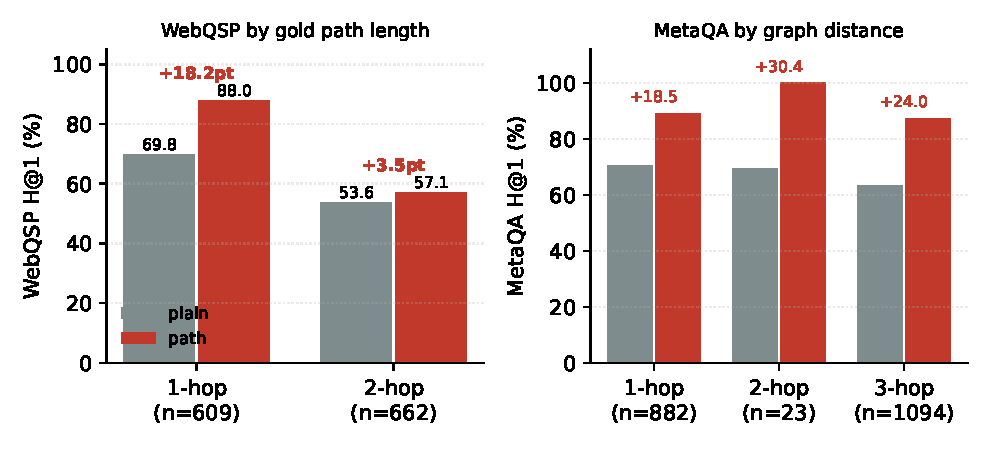
\includegraphics[width=\linewidth]{figures/fig7_pathlen.pdf}
\caption{Left: WebQSP split by the gold candidate's path length---the benefit concentrates on 1-hop questions. Right: MetaQA by graph distance; every distance gains.}
\label{fig:pathlen}
\end{figure}

\paragraph{Content controls.}
Replacing each candidate's path with random relations of the same length drops WebQSP H@1 from 56.18 to 39.52; masking the candidate name while keeping the path drops it to 42.10, below the no-path fused baseline (48.30). Both are out-of-distribution inputs, so we read them as directional evidence: the gain comes from reading the correct path \emph{together with} the entity, not from extra tokens.

\paragraph{Cross-KG transfer.}
A WebQSP-trained verifier scores 29.2\% on MetaQA and 24.1\% on CWQ, i.e.\ it does not transfer zero-shot across KGs; re-fitting costs about seven minutes per dataset and recovers each domain's own ceiling (88.8 on MetaQA with the twin recipe, and $+1.9$ over no path on CWQ, \S\ref{sec:boundary}). A data-scale sweep (25\%/50\%/100\% of the training groups) gives 50.46/52.43/54.89, so a quarter of the data still beats the plain verifier by 8.5 points. The method is therefore \emph{portable across retrievers} and \emph{cheap to re-fit across KGs}, not zero-shot.

\subsection{Ablations and negative results}
\label{sec:neg}

\begin{itemize}
\item \textbf{Renderings.} Full relation chain / namespace-stripped / natural-language sentence / chain with intermediate entities: 54.89 / 55.87 / 56.48 / 56.36. The method does not depend on dataset-specific relation naming, and intermediate entities add nothing.
\item \textbf{Backbone control.} Same pool, same prompt, same recipe: RWKV-7-Goose 191M 55.50, GPT-2 124M 48.37, Pythia-160M 46.28. RWKV-7-Goose was pre-trained on more tokens, so this is not a pure architecture comparison.
\item \textbf{Answer-type constraints} cost 0.43 points; the path-conditioned verifier already captures type implicitly.
\item \textbf{Two-stage head} is below the single fine-tuned head in 4/5 seeds (58.29 vs.\ 58.46 mean) and was removed.
\item \textbf{Beam 400} is negative ($-0.7$); \textbf{max-children} 128$\to$512 changes nothing, refuting a recall-bound hypothesis.
\item \textbf{Hard negatives for the relation head} (raising the hard-negative fraction 0.2$\to$0.3) leave validation in-candidate recall unchanged (0.7796$\to$0.7796); stopped before test.
\item \textbf{Top-15$\to$25 relations} gives 57.13 vs.\ 57.60 over three seeds: negative, the pipeline is at its plateau.
\item \textbf{Validation-based tuning} is impossible: validation pools are $\le$100 candidates and validation and test rank parameters in opposite directions.
\end{itemize}

%% ---------------------------------------------------------------- 6
\section{Limitations}
\label{sec:limitations}

\begin{enumerate}
\item \textbf{Accuracy is not the selling point.} NSM (110M, 68.7\% WebQSP) dominates us on the parameter--accuracy plane, and KGT5 (60M, 56.1\%) is more parameter-efficient.
\item \textbf{Not a new architecture.} The deployed system is a shared recurrent backbone, a path-conditioned prompt and a linear head.
\item \textbf{The boundary is narrow.} On WebQSP the benefit concentrates on 1-hop questions ($+18.2$) while 2-hop questions gain only 3.5 points, and on CWQ the twin-controlled gain is 1.9 rather than 6.6; a coarse relation-type summary is needed to obtain it there.
\item \textbf{MetaQA is easy}: pool oracle 99.8\%, so it measures ranking, not open-domain recall.
\item \textbf{Insertion is not free}: $+26$\,ms batched, $+428$\,ms if candidates are scored serially; $+2.2$\,GB.
\item \textbf{Cross-KG zero-shot fails}; per-dataset re-fitting is required.
\item \textbf{Portability has a measured boundary.} We test two heterogeneous hosts. On RoG-7B, a generative retriever with 16--30 noisy candidates per question, the verifier transfers without retraining ($+5.2$). On GNN-RAG's ReaRev-WebQSP, whose pool holds 8.1 candidates and already contains the gold answer for 88.8\% of questions, the same verifier \emph{loses} 1.9 points to the host's own in-domain scorer, and re-fitting on the host's split does not fix it (\S\ref{sec:portable-results}). The supported claim is therefore ``any retriever whose candidate set is recall-oriented'', not ``any retriever''; a strong GNN that has already ranked a short list is a host we do not improve.
\item \textbf{Sharing one backbone with the walker} saves 191M parameters; the joint fine-tuning stage that accompanies it is a confound, so we do not claim an accuracy benefit from sharing per se.
\item \textbf{No distillation from an LLM is used}; a 7B teacher could plausibly add points, but it would undercut the paper's premise.
\end{enumerate}

\paragraph{Threats to validity.}
(i) All test numbers are single-shot under a pre-registered protocol; ablation recipes differ slightly from the deployed checkpoint and are therefore compared only within one fixed recipe. (ii) The 2-hop and MetaQA 2-hop buckets are small ($n=662$ and 23) and we report them descriptively. (iii) Latency depends on batching policy, so both the batched and the serial figure are reported. (iv) The backbone comparison is confounded by pre-training data.

%% ---------------------------------------------------------------- 7
\section{Conclusion}
\label{sec:conclusion}

The expensive part of LLM-based KGQA is generating paths; the useful part may simply be \emph{showing the path to a ranker}. A 0.19B path-conditioned verifier, trained in minutes, portable to recall-oriented retrievers and re-fittable per KG, improves a 7B retriever's top-1 accuracy by 5.2 points (18.9 when the retriever over-generates) at a cost of 26 ms and 2.2 GB, and can even buy back retrieval budget at narrow beam widths. We hope the measurement of how far the signal reaches---path length, positive density, a relation-type summary that suffices on a large-vocabulary KG, and a second host it does not help---is as useful as the gains.

\begin{acks}
Omitted for double-blind review.
\end{acks}

\bibliographystyle{ACM-Reference-Format}
\bibliography{refs}

\appendix

\section{Hardware consistency}
\label{app:hw}
Three stored checkpoints were re-evaluated on a second GPU (RTX 5090, sm\_120). Path verifier: 0.5618 $\rightarrow$ 0.5630; final system seed 42: 0.5833 $\rightarrow$ 0.5827; MetaQA path: 0.8820 $\rightarrow$ 0.8855. Repeat runs on the same GPU are bit-identical, so the residual spread ($\le0.4$ points) is a cross-architecture kernel effect.

The revision experiments (external rerankers, MetaQA full-set twins, reader study) were run on an RTX 3090 with a different software stack (torch 2.5.1/CUDA 12.1 vs.\ 2.8.0/CUDA 12.8, same \texttt{fla} 0.2.1 and transformers 4.49.0). Two checks separate hardware from retraining. First, the published plain baseline reproduces at 44.38 vs.\ 44.19 (+0.19) with the same in-pool oracle (0.7554 vs.\ 0.7548), so hardware is not the source of drift. Second, rebuilding the whole chain there (relation head and path verifier retrained, same seeds and recipe) gives 56.42 vs.\ 54.89 (+1.5): re-training moves absolute accuracy more than hardware does. Every comparison in a table is therefore computed within one GPU and one software stack, and no cross-stack difference is used as evidence. Latency numbers remain those of the RTX 4090 machine.

\section{Long-context state reuse (negative)}
\label{app:longctx}
With a 0.19B RWKV-7 the recurrent state can be carried across dialogue turns. In a 30-question pilot ($H\in\{0,16,32\}$ turns), state-based reuse matched concatenation in accuracy exactly (0.500/0.500 at $H=16$; 0.467/0.467 at $H=32$), confirming the implementation, but was slower at batch size 1 (952 vs.\ 610 ms/query at $H=16$) because per-candidate kernel launch dominates, and history \emph{reduced} accuracy (53.3\%$\to$46.7\%) since the verifier was never trained with history. Reuse therefore needs multi-turn training data and batched state expansion.

\section{Reproducibility}
\label{app:repro}
All datasets are public. The pipeline is: mine candidates $\rightarrow$ build path groups $\rightarrow$ train the listwise verifier (2 epochs) $\rightarrow$ evaluate end-to-end once; a full WebQSP run takes about 40 minutes on one RTX 4090 (20 head, 7 verifier, 13 evaluation). Code, checkpoints, logs, the scripts that produce every number and figure, and the paired-test utilities are released in an anonymized repository (URL in the artifact field), together with the negative results so that they can be re-run rather than taken on trust. The pre-registered parameters of \S\ref{sec:protocol} are the defaults of the released evaluation script, so any deviation is visible in the command recorded next to each result file.

\end{document}
